% Slide 09: Project Timeline
\begin{frame}{Project Timeline}
    \framesubtitle{18-Month Roadmap}

    \begin{center}
        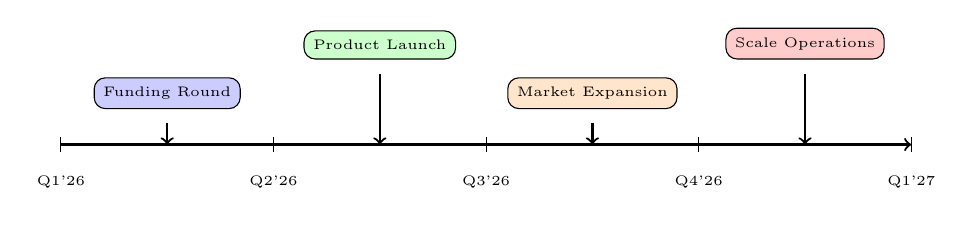
\begin{tikzpicture}[scale=0.9]
            % Timeline axis
            \draw[->,thick] (0,0) -- (12,0);

            % Quarter markers
            \foreach \x/\quarter in {0/Q1'26,3/Q2'26,6/Q3'26,9/Q4'26,12/Q1'27}
            {
                \draw (\x,0.1) -- (\x,-0.1);
                \node[below] at (\x,-0.3) {\tiny \quarter};
            }

            % Milestones
            \node[draw,fill=blue!20,rounded corners,above] at (1.5,0.5) {\tiny Funding Round};
            \node[draw,fill=green!20,rounded corners,above] at (4.5,1.2) {\tiny Product Launch};
            \node[draw,fill=orange!20,rounded corners,above] at (7.5,0.5) {\tiny Market Expansion};
            \node[draw,fill=red!20,rounded corners,above] at (10.5,1.2) {\tiny Scale Operations};

            % Arrows to timeline
            \draw[->,thick] (1.5,0.3) -- (1.5,0);
            \draw[->,thick] (4.5,1) -- (4.5,0);
            \draw[->,thick] (7.5,0.3) -- (7.5,0);
            \draw[->,thick] (10.5,1) -- (10.5,0);
        \end{tikzpicture}
    \end{center}

    \vspace{0.5cm}

    \begin{columns}[t]
        \begin{column}{0.48\textwidth}
            \textbf{Phase 1: Foundation (Q1-Q2)}
            \begin{itemize}
                \item Secure Series A funding
                \item Expand development team
                \item Complete beta testing
                \item Launch MVP to market
            \end{itemize}
        \end{column}

        \begin{column}{0.48\textwidth}
            \textbf{Phase 2: Growth (Q3-Q4)}
            \begin{itemize}
                \item Scale to 500+ customers
                \item Enter 3 new markets
                \item Achieve profitability
                \item Prepare for Series B
            \end{itemize}
        \end{column}
    \end{columns}
\end{frame}
